\begin{figure*}[t]
    \centering
    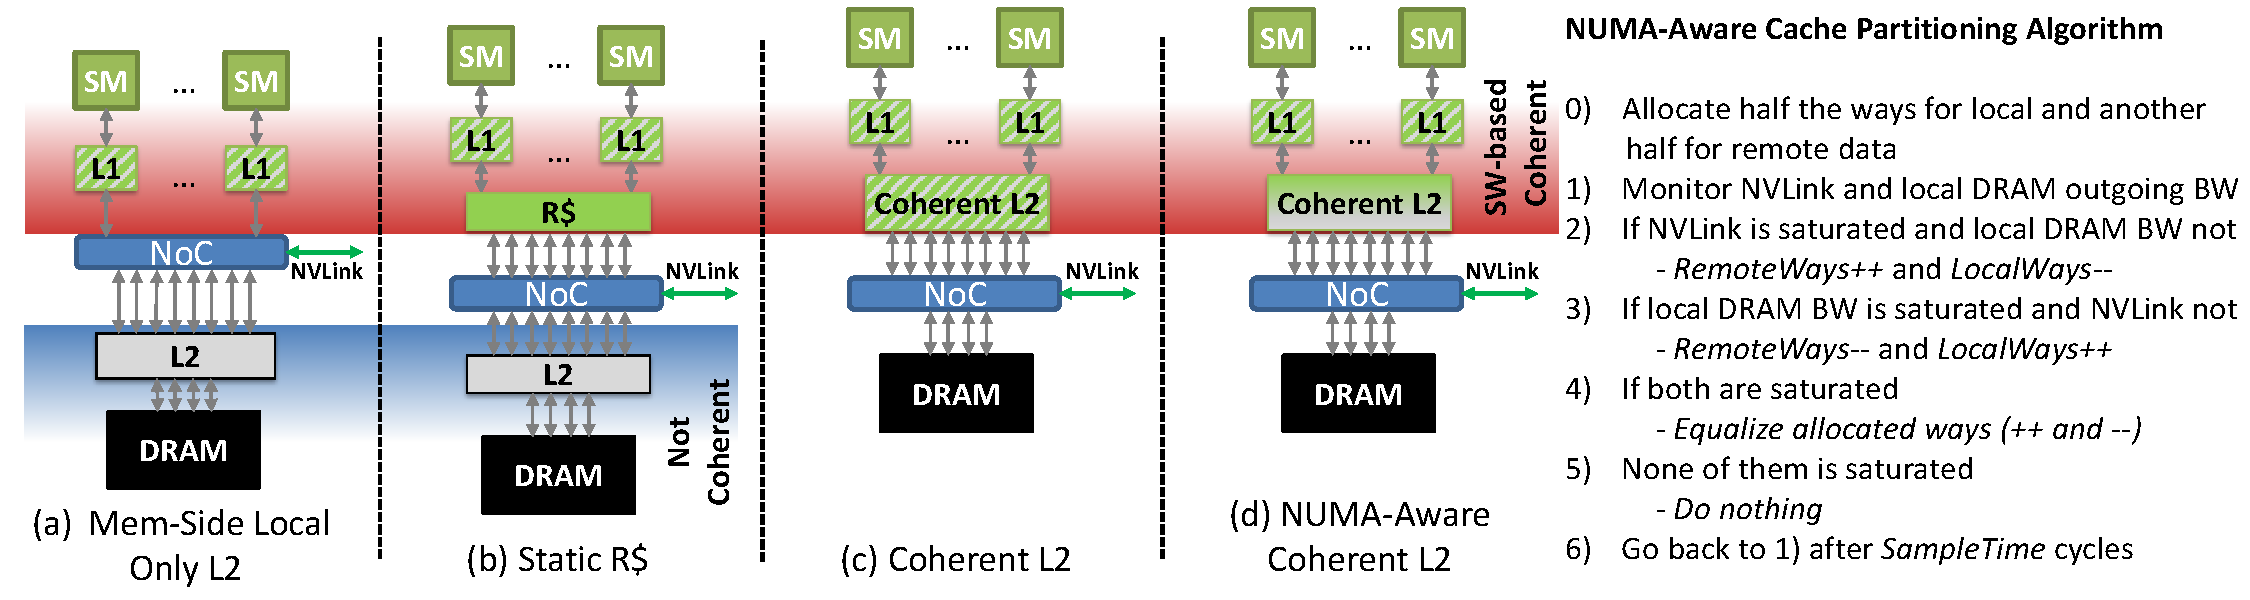
\includegraphics[width=1.0\textwidth]{figures/cache_configurations_static_dynamic.pdf}
    \caption{Potential L2 cache organizations to balance capacity between remote and
    local NUMA memory systems.}
    \label{fig:cacheorg}
\end{figure*}

\section{NUMA-Aware Cache Management}
\label{caching}
In Section~\ref{sec:interconnect} we have shown that inter-socket bandwidth is one
of the most important factors in achieving scalable NUMA GPU performance. By
dynamically retraining the link to support asymmetric bandwidth configurations,
rather than a static uniform balance, we are able to improve the average performance
of applications by 14\%.  This improvement comes not from increasing the
absolute bandwidth of the link, but by using the existing link more efficiently.
Unfortunately, because either the outgoing or incoming links must be underutilized
for us to reallocate that bandwidth to the saturated link, if both incoming and
outgoing links are saturated, this technique yields little improvement.
To improve performance in situations where dynamic link balancing is not effective,
system designers can increase link bandwidth, which is very expensive,
or try and decrease the amount of traffic that crosses the low bandwidth
communication channels.  To decrease off-chip memory traffic, architects typically
turn to caches to capture locality whenever possible.

GPU cache hierarchies differ from traditional CPU hierarchies where in they 
are not supported by strong hardware coherence protocols~\cite{Singh2013}. 
They also differ from CPU protocols in that caches designed for a single 
uniform memory access GPU may be both processor side (where some form of 
coherence is typically necessary) or they may be memory side (where coherence 
is not necessary).  As described in Table~\ref{tab:setup} and shown in 
Figure~\ref{fig:cacheorg}(a), a GPU today is typically composed of relatively 
large SW managed coherent L1 caches that are physically proximal to the SM's, 
while a relatively small, distributed, non-coherent L2 cache resides memory 
side close to the memory controllers.  This organization works well for GPUs 
because their SIMT processor designs often allow for significant coalescing 
of requests to the same cache line, so having large L1 caches reduces the 
need for global crossbar bandwidth.  By then placing the L2 caches 
memory-side, they do not need to participate in the coherence protocol.  
Because of the fine grained interleaving of physical memory addresses across 
memory channels, the L2 caches are inherently load balanced.

\begin{figure*}[t]
    \centering
    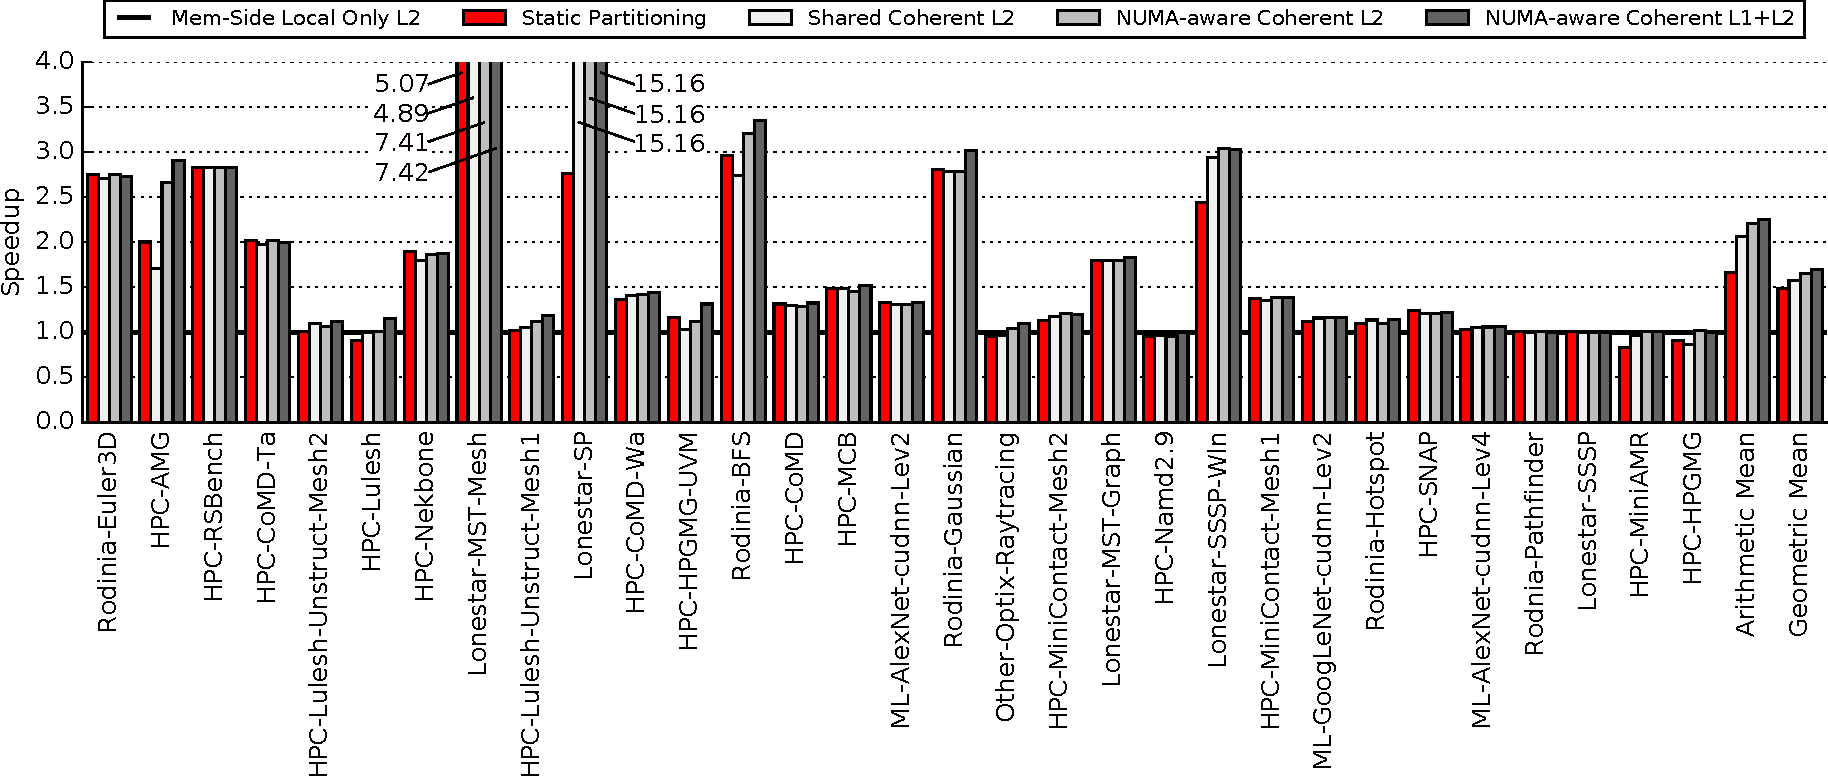
\includegraphics[width=1.0\textwidth]{figures/plot_merged_cache_WB.pdf}
    \caption{Performance of NUMA-aware dynamic cache partitioning in a 4-socket
	GPU compared to memory-side L2 and previously proposed static partitioning.}
    \label{fig:dynamiccaching}
        \vspace{-.2in}
\end{figure*}

\subsection{Cache Partitioning Options}
In NUMA-designs interleaving memory references across the low bandwidth NUMA 
interconnections results in poor performance, as shown in 
Figure~\ref{fig:motivation}. Similarly, in NUMA GPUs utilizing the 
traditional memory side L2 caches that depend on fine grained memory 
interleaving is a bad decision because these memory side caches are not able 
to cache remote memory, and thus cannot reduce NUMA interconnect traffic.  
Previous work has proposed that GPU L2 cache capacity should be split between 
memory-side caches and a new processor-side L1.5 cache that is an extension 
of the GPU L1 caches~\cite{Arunkumar2017} for caching remote data only (we 
denote them as Remote caches here). By balancing this capacity between local 
and remote caches (R\$ caches) they limit the need for invalidating the entire 
L2 cache capacity when extending the GPU coherence into the R\$ cache while still 
minimizing crossbar bandwidth. An example of this organization is shown in 
Figure~\ref{fig:cacheorg}(b). 

Static designs that allocate cache capacity to local memory, remote memory, 
or any other balance, may achieve reasonable performance but they lack 
flexibility. Much like application phasing was shown to affect NUMA bandwidth 
needs, the ability to dynamically share cache capacity between local and 
remote memory has the potential to improve performance under several 
situations. First, when application phasing results in some sockets within 
the NUMA GPU to access data locally, while others are accessing remote data, 
as shown in Figure~\ref{fig:link-motivation}, allowing the entire L2 to cache 
both local and remote data should outperform any static policy. Second, while 
we show that many applications will be able to completely utilize large 
NUMA GPUs, this may not always be the case. GPUs within the data center are 
being virtualized and there is on-going work to support concurrent execution 
of multiple processes within a single GPU~\cite{park2015chimera, 
lin2016enabling}. If a large NUMA GPU is sub-partitioned, it is intuitive 
that system software attempt to partition it along the NUMA boundaries so 
that a single small application need not endure NUMA effects. To effectively 
capture locality in such a situation, NUMA-aware GPUs need to be able to 
flexibly move from 100\% local to 100\% remote caching at runtime, rather 
than be statically partitioned at design time. 

Static L2 cache partitioning between local and remote data results in a GPU 
cache organization in which the L1 caches contain both local and remote data 
but the GPU L2 cache(s) will contain only local or remote data.  To-date, 
single socket GPUs have not moved their memory-side caches to processor side 
because the overhead of cache invalidation (due to coherence) is an 
unnecessary performance penalty, with no performance upside to justify the 
cost. However in a multi-socket NUMA GPU, rather than statically 
partitioning the L2 cache at design time, the entire L2 cache could be made 
an extension of the L1 and both local and remote data could dynamically 
contend for capacity. Figure~\ref{fig:cacheorg}(c) shows a configuration with 
such coherent L2 cache. While conceptually simple, allowing both remote and 
local memory accesses to contend for cache capacity in a NUMA system is flawed.

In non-NUMA systems, performance is maximized by optimizing for cache 
hitrate, which minimizes off-chip memory system bandwidth. In NUMA systems 
however, not all cache misses have the same relative cost, and thus 
performance impact. A cache miss to a NUMA-local memory address will have a 
smaller cost (in both terms of latency and bandwidth) than a cache miss to a 
NUMA-remote memory address. Thus, it should be beneficial to dynamically 
skew cache allocation policy to preference caching of remote memory over 
local data when it is determined the system is bottlenecked on NUMA bandwidth.

We propose that rather than allowing both the L1 and L2 caches to be 
contended by local and remote memory accesses, both levels of the GPU cache 
hierarchy become NUMA-aware and dynamically adjust their cache resources to 
preference caching of remote NUMA data when it is determined that the NVLink 
bandwidth in our hypothetical GPU is oversubscribed. We do this by 
implementing the NUMA-aware cache partitioning algorithm, similar to the 
adaptive NVLink switching policy. Cache organization and a brief summary is 
shown on Figure~\ref{fig:cacheorg}(d). 

At the beginning, we allocate one half of the cache ways for local, and 
another half for caching remote data (Step \circled{0}). After the sampling 
period, we collect the bandwidth values on the outgoing NVLink and local 
memory channels. Link utilization above 99\% is considered to be saturated 
(Step \circled{1}). In case where NVLink is saturated and local memory 
bandwidth is not, the partitioning algorithm tries to reduce remote traffic 
by assigning one way from a set of local ways, and allocating it to a set of 
remote ways (Step \circled{2}). If it is a write-back cache (only L2), dirty 
lines from the assigned way are written back to the backing memory. 
Similarly, if the local memory BW is saturated and NVLink is not, the policy 
takes one way from remote, and allocates it now to a set of local ways (Step 
\circled{3}). That way, our NUMA-aware cache partitioning algorithm reduces 
remote or local link utilization depending on which one of the two stands as 
a performance bottleneck. In case where both NVLink and local memory channels 
are saturated, we gradually equalize the number of ways assigned for remote 
and local cache lines (Step \circled{4}). Finally, if none of the links have 
been saturated, the policy takes no action (Step \circled{5}).

\begin{figure}[t]
    \centering
    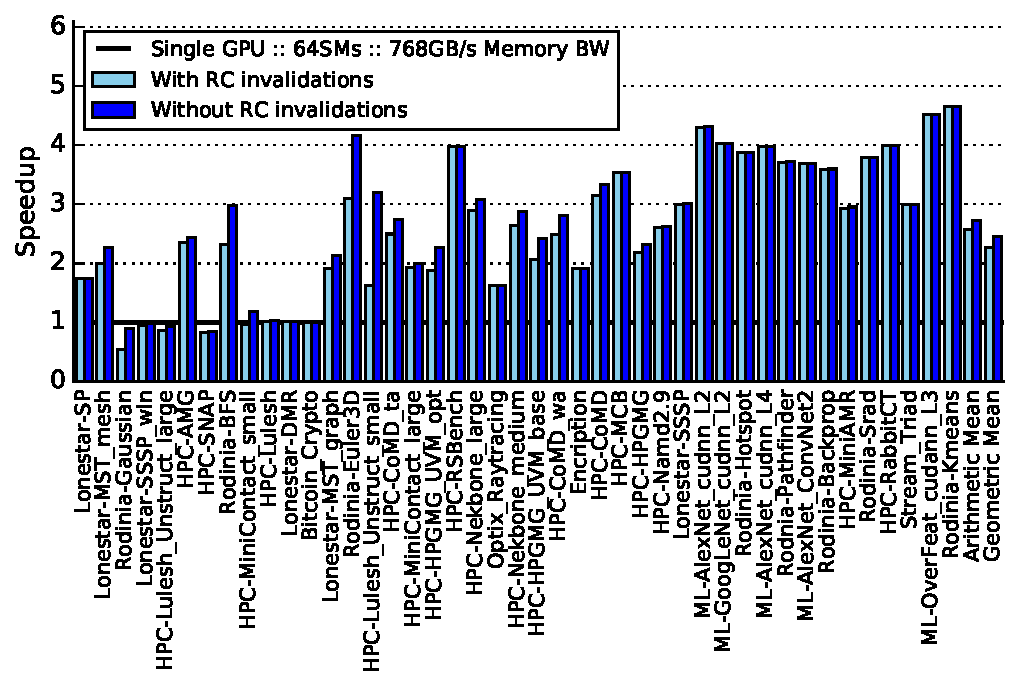
\includegraphics[width=1.0\columnwidth]{figures/plot_no_inval_WB.pdf}
    \caption{Performance overhead of extending current GPU software based coherence
    into the GPU L2 caches.}
    \label{fig:invalidations}
    \vspace{-.2in}
\end{figure}

\begin{figure*}[tp]
    \centering
    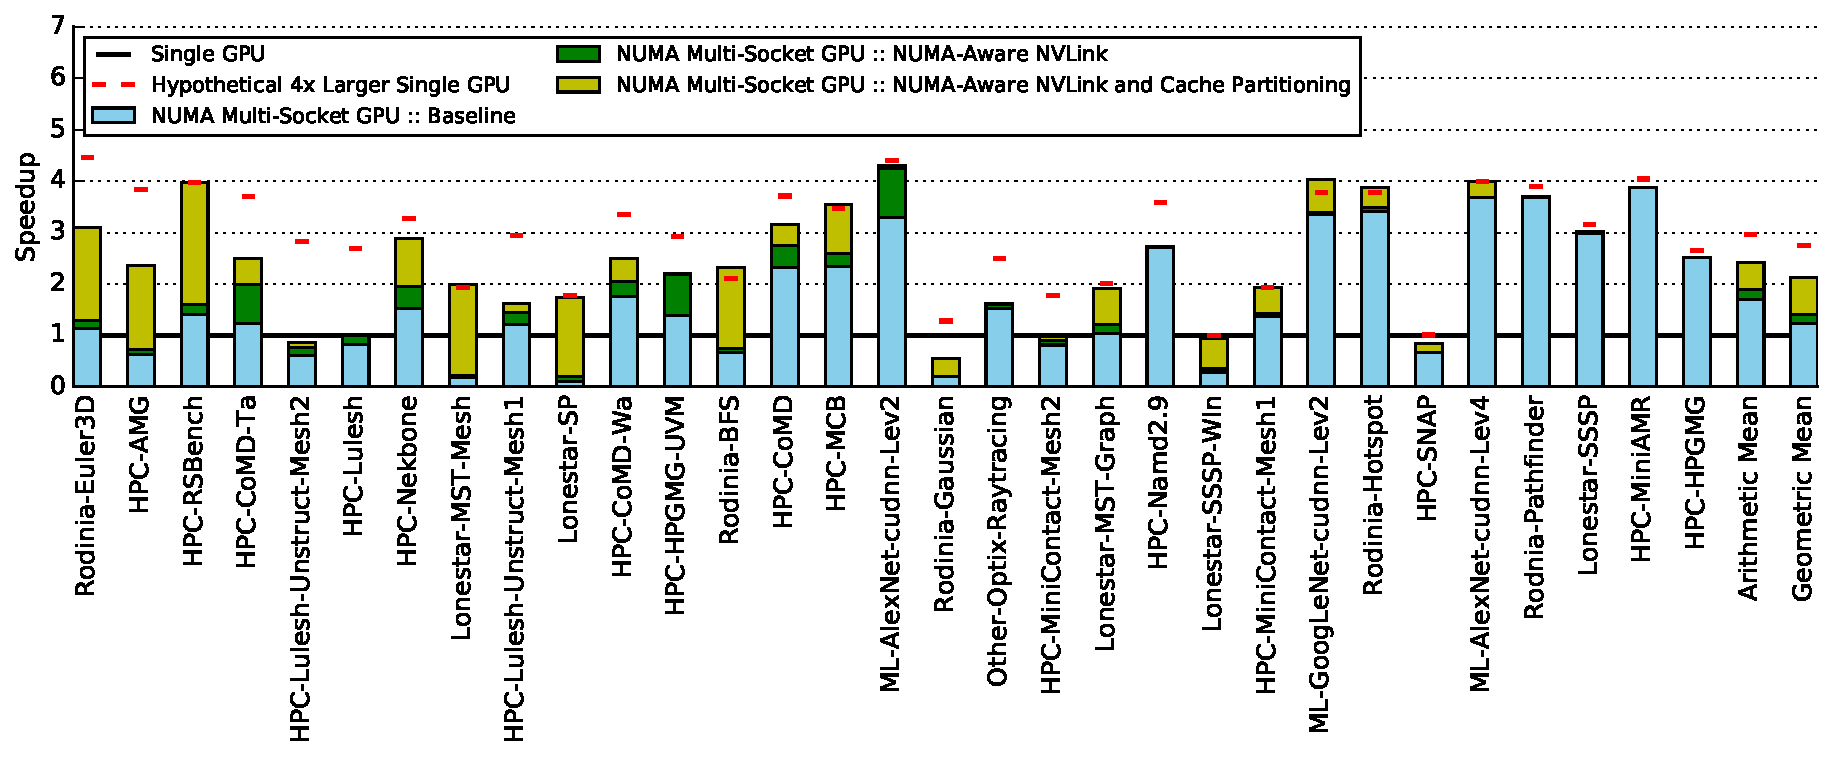
\includegraphics[width=1.0\textwidth]{figures/plot_final_speedup_WB_nvlink_first.pdf}
    \caption{Performance of a 4-socket NUMA-aware GPU compared to a single GPU and a hypothetical 4x large single GPU with proportionally scaled resources.}
    \label{fig:combined}
    \vspace{-.2in}
\end{figure*}

\subsection{Results}

Figure~\ref{fig:dynamiccaching} compares the performance of different cache 
partitioning configurations. Our baseline is a 4-socket GPU with memory side, 
local-only L2 caches. With \emph{red bars}, we show speedup gained by equally 
splitting the L2 cache budget, between the gpu-side R\$ which caches only 
remote data, and mem-side L2. Previous work reports this as the best static 
L2 partitioning scheme~\cite{Arunkumar2017}. Indeed, this configuration 
improves the performance by 50\% on average, although for some benchmarks, 
like \texttt{HPC-MiniAMR} and \texttt{HPC-HPGMG} it hurts the performance by 
up to 10\%. Those workloads stress local memory bandwidth and have negligible 
inter-socket traffic, thus lowering the mem-side L2 capacity creates the 
bottleneck. \emph{Light gray} bars we show the results for a configuration with 
coherent L1 and L2 caches where both local and remote data contend for the 
available capacity. On average, this solution outperforms static cache 
partitioning, although for \texttt{HPC-HPGMG} results in a decrease of 
performance.

Finally, the \emph{dark gray} bar shows our proposed NUMA-aware cache 
partitioning policy. All caches in the NUMA-aware multi-socket GPU system are 
able to independently change their local behavior based on the hardware 
counters monitoring the outgoing NVLink and local memory bandwidth. The 
flexibility of our proposal and its ability to adapt at runtime, results in 
the best possible configuration a particular benchmark can exploit. For the 
workloads on the left side of Figure~\ref{fig:dynamiccaching} which fully 
saturate the NVLink bandwidth, NUMA-aware dynamic policy arrange the L1 and 
L2 caches to be entirely used as a remote-only cache. Unlike the conclusions 
of the previous work, allocating 100\% of the cache to remote data is by far 
the highest performing configuration for these applications. The difference 
in this conclusion is likely due to the fact that their intra-GPU crossbar 
has significantly more bandwidth than our multi-socket NUMA links, and thus 
we need to dedicate more (all) of the GPU's L1 and L2 capacity to caching 
remote data, despite the fact that SW based cache coherence will now 
effectively flush the entire L2 cache on all GPUs when those operations 
occur. Moreover, workloads on the right side expose good locality, thus 
prefer L1 and L2 caches to store (mostly) local data, something that 
NUMA-aware policy can adapt to. We see that dynamic partitioning can improve 
average GPU performance by 71\% compared to the memory side L2, and 21\% 
compared to the static cache partitioning. 

Extending NUMA-aware dynamic cache mechanism to L1 caches results in an 
interesting observation. In situations where both L1 and L2 caches end up as 
remote-only (finding that NVLink is saturated while local memory bandwidth is 
not), we have detected performance degradation for some benchmarks. With no 
local ways left inside the L1 caches, local memory accesses start missing in 
the L1, reserving all MSHR entries. Running out of available MSHR entries 
blocks the entire cache thus none of the memory accesses can be served, 
reducing the number of available warps to keep an SM busy. On the other side, 
with L2 caches being also remote-only, these local memory misses are now 
propagated further to the local memory. That way, the execution time 
increases without enough parallelism to hide prolonged memory accesses. To 
mitigate this problem, we tunned our NUMA-aware policy for L1 caches, by not 
allowing them to allocate all available ways to either local or remote data, 
but keep at least one way for any of both. 

\subsection{Extending the Coherency to L2 Caches}
When extending the software controlled GPU coherence protocol into the GPU L2 
caches, L1 coherence operations (flushes) must also be extended into the GPU 
L2 caches.  To understand the impact of these coherence operations on our 
dynamic cache performance we evaluated a hypothetical L2 cache which does not 
need to perform these coherence operations.  This experiment approximates a 
speed of light coherence implementation in which caches are still coherent 
but there is no cost for maintaining that coherence. In a 4-socket NUMA GPU 
with 64 SMs per GPU we observe that the coherence overhead of current 
software based GPU coherence is only 10.4\%. We conclude that despite some 
coherence overheads, the benefit of dynamic NUMA-aware coherent L2 caches on 
multi-socket GPUs will be required to maximize both performance and GPU 
flexibility. 


